%!TEX root = ../Thesis.tex

\section{Long-Short Term Memory}

In the case of the Recurrent Neural Network the internal state $b_h^t$ must be updated in each iteration. This mean the effect of some input $x_i^{t_0}$ on $b_h^{t_0}$, will decay as $t \gg t_0$. This issues is addressed in the Long-Short Term Memory Model (LSTM) by taking inspiration from a computer memory cell.

A computer memory cell can either be written to, read from or reset. On the most basic level memory cell are binary, not just in terms of what can be stored by also in terms of the 3 operations. Either the memory cell is completely reset or not reset, either completely read from or not read from and similarly for witting. This from a mathematical perspective all these operations becomes threshold functions, which are not differentiable or continues. This makes it impractical to use in a neural network context, as these are optimized using gradient decent. The solution is not to use threshold function but a combination of continues and differentiable activation functions, such as sigmoid or the hyperbolic tangent function.

\subsection{The memory block}

\begin{figure}[h]
	\centering
	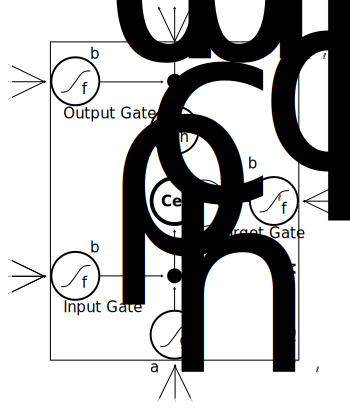
\includegraphics[scale=0.7]{theory/lstm-block}
	\caption{Visualization of the continues and differentiable memory block.}
	\label{fig:theory:lstm:lstm-block}
\end{figure}

Consider Figure \ref{fig:theory:lstm:lstm-block}. The arrows at the bottom makes the \textit{input} and corresponds to $a_h^t$. The top arrows contains the \textit{output} and corresponds the $b_h^t$. The \textit{input gate} controls how much the input affects the memory \textit{cell}. Similarly the \textit{forget gate} controls how much the of cell values should be kept. For example if the \textit{input gate} is $0$ and the \text{forget gate} is $1$, then the cell value won't change. Or if they are both $0.5$ then an average of the input and the current cell value with be stored. Note that the \textit{input gate} and \textit{forget gate} don't need to sum to one, thus the cell can hold any value. However a transformation ($h$) is applied to the new cell value so the total \textit{output} can be constrained, though in some cases $h$ is the identity function. The transformed cell value is finally controlled by the \textit{output gate}. If the \textit{output gate} is $0$ then the finial \textit{output} will also be $0$, if the \textit{output gate} is $1$ then the transformed cell value is the final \textit{output}.

\subsection{Forward pass}

\begin{equationbox}[H]
Input Gates: -- Why is the internal cell state $s_c^{t-1}$ used in other cells.
\begin{equation*}
\begin{aligned}
a_\iota^t &= \sum_{i=1}^I w_{i \iota} + \sum_{h=1}^H w_{h \iota} b_h^{t-1} + \sum_{c=1}^C w_{c \iota} s_c^{t-1} \\
b_\iota^t &= f(a_\iota^t)
\end{aligned}
\end{equation*}
Forget Gates:
\begin{equation*}
\begin{aligned}
a_\phi^t &= \sum_{i=1}^I w_{i\phi} + \sum_{h=1}^H w_{h \phi} b_h^{t-1} + \sum_{c=1}^C w_{c \phi} s_c^{t-1} \\
b_\phi^t &= f(a_\phi^t)
\end{aligned}
\end{equation*}
Cells: -- How should the subscript be understood
\begin{equation*}
\begin{aligned}
a_c^t &= \sum_{i=1}^I w_{i c} x_i^t + \sum_{h=1}^H w_{h c} b_h^{t-1} \\
s_c^t &= b_\phi^t s_c^{t-1} + b_{\iota}^t g(a_c^t)
\end{aligned}
\end{equation*}
Output Gates: -- Why $s_c^t$ and not $s_c^{t-1}$
\begin{equation*}
\begin{aligned}
a_\omega^t &= \sum_{i=1}^I w_{i\omega} + \sum_{h=1}^H w_{h \omega} b_h^{t-1} + \sum_{c=1}^C w_{c \omega} s_c^t \\
b_\omega^t &= f(a_\omega^t)
\end{aligned}
\end{equation*}
Cell Output: -- Should $b_c^t$ not be $b_h^t$
\begin{equation*}
\begin{aligned}
b_c^t = b_\omega^t h(s_c^t)
\end{aligned}
\end{equation*}
\caption{Forward equations for a single layer LSTM network.}
\end{equationbox}
